\documentclass[11pt,a4paper]{article}

%, Page Geometry & Layout ,
\usepackage[margin=1in]{geometry}
\usepackage[utf8]{inputenc}
\usepackage[T1]{fontenc}
\usepackage{lmodern}

%, Core Math & Symbols ,
\usepackage{amsmath,amssymb,amsfonts,amsthm}

%, Graphics, Tables & Formatting ,
\usepackage{graphicx}
\usepackage{booktabs}
\usepackage{microtype}
\setlength{\emergencystretch}{2em}
\usepackage{setspace}
\setstretch{1.12}

%, Tables ,
\usepackage{array}
\usepackage{multirow}
\usepackage{tabularx}
\renewcommand{\arraystretch}{1.15}
\setlength{\tabcolsep}{6pt}
\newcolumntype{R}{>{\raggedleft\arraybackslash}X}
\newcolumntype{L}{>{\raggedright\arraybackslash}X}
\newcommand{\tabfont}{\footnotesize}
\newcommand{\thead}[1]{\footnotesize\textbf{#1}}

%, Captions ,
\usepackage{caption}
\captionsetup{font=small, labelfont=bf}

%, Lists ,
\usepackage{enumitem}
\setlist[itemize]{leftmargin=1.5em,itemsep=2pt,topsep=4pt,parsep=0pt}
\setlist[enumerate]{leftmargin=1.8em,itemsep=2pt,topsep=4pt,parsep=0pt}

%, Colors ,
\usepackage[table,dvipsnames]{xcolor}
\definecolor{arblue}{HTML}{2A78D6}
\definecolor{dgorange}{HTML}{EB6834}
\definecolor{llaqua}{HTML}{1BAF7A}
\definecolor{linkc}{HTML}{1B3A5C}

%, Hyperlinks & Metadata ,
\usepackage[
    colorlinks=true,
    linkcolor=linkc,
    citecolor=linkc,
    urlcolor=linkc,
    pdfauthor={Aleksandr Kaigorodov},
    pdftitle={When Block-Diffusion Language Models Are Faster},
    pdfsubject={Block-structured decoding cost analysis},
    pdfkeywords={diffusion LLM, block decoding, latency, structured output}
]{hyperref}

%, Model shorthands ,
% NB: \ARthree renders AR-30B (the name is an AR-3B-era leftover).
\newcommand{\ARthree}{\textsc{ar-30b}}
\newcommand{\DG}{\textsc{dg}}
\newcommand{\LLaDA}{\textsc{llada-8b}}

%, Macros (numbers from results/) ,
% =============================================================================
%  macros.tex — every number the paper cites, in one place.
%
%  Rule: every measurement is a macro here, and the comment on its line names
%  the artifact it was read from. Section files may hardcode derived ratios
%  (e.g., 2.5×) and structural constants (e.g., 12 fields, $K{=}8$) for
%  readability, but raw measurements (latencies, F1 scores, energy) must be
%  macros. paper/verify_numbers.py checks provenance blocks and decimal-place
%  policy; the figure builder (paper/figures/make_figures.py) prints what it
%  plotted so the two can be diffed.
% =============================================================================

% --- Pinned stack -------------------------------------------------- (#57) --
\newcommand{\gpuModel}{NVIDIA A100 80GB PCIe}
% prompt_token_count in every DG cell (issue68_dg_L*.json, 42 files). The AR
% cells run shorter prompts (992); 1,077 is the DG figure the crossover is
% calibrated at. Was 1,047 -- a stale constant from docs/edr/005, no artifact.
\newcommand{\refPrompt}{1{,}077}

% --- Quality, 9-field vs 12-field ----- results/issue43_nine_field_f1.json --
\newcommand{\arThreeBFnine}{0.852}     % dense AR-3B (Qwen2.5-3B), L=256, 9-field, re-scored (#43)
\newcommand{\qualityGap}{0.000}        % |9-field difference|
\newcommand{\twelveGap}{0.041}         % 12-field difference, AR-favoured

% --- Cost laws ------------- results/anchors/*.json, results/issue68_*.json --
% AR-30B (arBase/arSlope/crossoverL): results/issue111_qwen3_serial_sweep.json
%   cost_law.{intercept_ms,slope_ms_per_token,crossover_L_star}.
%   Corrected serial-sweep artifact carries vLLM 0.25.1 provenance.
%   This fit uses cell means, not event medians; see v8 Section 2.
\newcommand{\arBase}{34.6}        % ms, AR-30B MoE serial intercept (Qwen3-30B-A3B)
\newcommand{\arSlope}{7.2}       % ms/token, AR-30B MoE serial decode slope
\newcommand{\dgBase}{378.8}       % ms, DG base at K=8
\newcommand{\dgStep}{119.5}       % ms, median of the 7 measured canvas steps
\newcommand{\dgStepLo}{113.1}     % ms, smallest measured step (1280->1536)
\newcommand{\dgStepHi}{122.6}     % ms, largest measured step (256->512)
\newcommand{\canvasLength}{256}   % tokens per canvas

% Anchors, five repeats each -------- results/anchors/anchor_remeasure.json --
% Per-event dispersion: n=2000 (issue #120, was n=300 where p99.9==max)
% results/anchors/dg_L256_r1_preds.jsonl, ar3b_L256_n2000_preds.jsonl
\newcommand{\arEventCV}{0.1}     % % CV over 2000 per-event latencies (AR-3B dense)
\newcommand{\dgEventCV}{16.9}
\newcommand{\arMaxMed}{1.03}      % max / median per-event latency (AR-3B dense)
\newcommand{\dgMaxMed}{3.07}

% --- Crossovers ------- derived from arBase/arSlope/dgBase above --------------
% NB: models/decision/procedure.py CONSTANTS updated to match (#113 0.5e).
\newcommand{\crossoverL}{48}       % tokens: (dgBase - arBase) / arSlope, serial mode
\newcommand{\crossoverLambda}{2.6} % ev/s: 1000 / dgBase (unchanged — DG base same)

% --- Input length, the second variable ------ results/issue44_*_sweep.json --
\newcommand{\inputSlopeRatio}{2.6} % dgInputSlope / arInputSlope (0.1/0.038)

% --- Base decomposition ------------------- results/issue44_dg_ksweep_K*.json --
\newcommand{\kfitBase}{296.1}      % ms, K-independent term (NOT interpretable as a floor; see #70)
\newcommand{\kfitSlope}{2.6}      % ms per denoising step
\newcommand{\kfitRsq}{0.49}
% Superseded: the fitted intercept (296.1) is not a measured floor. R^2=0.49
% and the curve saturates above K=16, so the linear term is a poor description.
% The 93.5%/6.5% split it produced over-attributes to the floor by ~5x.
% Replaced by two measurement-based bounds (issue #70):
% Floor share <=53% (from T(2)=201.7ms), denoising share >=32% (from canvas step 119.5ms).
% Values are hardcoded in Appendix 10 (appendix_decomp.tex).

% --- Batching ------------------- results/issue42_batching.json, appD, dInfer --
% NB: #42 was run on the dense AR-3B (Qwen2.5-3B-Instruct), NOT the AR-30B MoE.
% The AR-30B MoE multiplier is 24.7x (results/issue111_qwen3_batch_sweep.json).
\newcommand{\cacheOnMult}{42.8}    % dense AR-3B, prefix caching on   (#42)
\newcommand{\cacheOffMult}{26.8}   % dense AR-3B, prefix caching off  (#42)
\newcommand{\dgBatchVllmHi}{1.7}   % DG under vLLM, L=128 (lower bound)

% Energy values for v8 are bound to source artifacts below.

% --- Deployment pair ------ results/issue_evidence_ar1b_*.json, issue68_*.json --
\newcommand{\dgWeights}{52.0}          % GB, bf16

% --- Defect magnitudes ------------------------------ CHECKLIST.md, #65 -----
\newcommand{\defectOneFBefore}{0.779}
\newcommand{\defectOneFAfter}{0.844}
\newcommand{\defectTwoBefore}{1841.6}
\newcommand{\defectTwoAfter}{413.3}
\newcommand{\defectTwoRatio}{4.5}
\newcommand{\defectThreeBefore}{0.599}
\newcommand{\defectThreeAfter}{0.826}
\newcommand{\defectFourBefore}{0}
\newcommand{\defectFourAfter}{100}
\newcommand{\rambleRate}{96}      % % of AR outputs with >1 JSON object at L=512

% --- Truncation regime -------------------------- results/issue43/*.json -----
\newcommand{\arFOneTwentyEight}{0.669}   % AR-3B (dense) 9-field F1 at L=128
\newcommand{\dgFOneTwentyEight}{0.311}   % DG    9-field F1 at L=128
\newcommand{\arValidTwentyEight}{66.7}   % AR-3B (dense) schema-valid % at L=128
\newcommand{\dgValidTwentyEight}{1.0}    % DG schema-valid % at L=128

% --- Generalisation to HDFS ---------------------- results/issue67_*.json ----
\newcommand{\hdfsStep}{120.5}     % ms, DG canvas step on HDFS
\newcommand{\bglStep}{118.5}      % ms, DG canvas step on BGL (same cells)

% --- Canvas tuning -------------------------- results/issue66_canvas_*.json --
\newcommand{\canvasOneTwentyEightBase}{368.5}  % ms at canvas=128
\newcommand{\canvasOneTwentyEightFone}{0.864} % 9-field F1 at canvas=128

% --- K as a runtime quality knob --------- results/issue44_dg_ksweep_K*.json --
\newcommand{\kFourPninetynine}{394.3} % ms
\newcommand{\kFourFone}{0.790}
\newcommand{\kEightFone}{0.853}


% --- v8 audited primary-pair statistics and corrected energy ---
\newcommand{\arMedian}{924.4} % results/anchors/ar30b_stats.json ar30b_bgl.p50_ms
\newcommand{\arCiLo}{918.2} % results/anchors/ar30b_stats.json ar30b_bgl.p50_ci_95.0
\newcommand{\arCiHi}{926.5} % results/anchors/ar30b_stats.json ar30b_bgl.p50_ci_95.1
\newcommand{\arPninetyNine}{1400.4} % results/anchors/ar30b_stats.json ar30b_bgl.p99_ms
\newcommand{\arThirtyCV}{12.25} % results/anchors/ar30b_stats.json ar30b_bgl.cv_pct
\newcommand{\dgMedian}{379.7} % results/anchors/ar30b_stats.json dg_bgl.p50_ms
\newcommand{\dgCiLo}{379.1} % results/anchors/ar30b_stats.json dg_bgl.p50_ci_95.0
\newcommand{\dgCiHi}{380.4} % results/anchors/ar30b_stats.json dg_bgl.p50_ci_95.1
\newcommand{\dgPninetyNine}{490.7} % results/anchors/ar30b_stats.json dg_bgl.p99_ms
\newcommand{\dgThirtyCV}{16.92} % results/anchors/ar30b_stats.json dg_bgl.cv_pct
\newcommand{\hdfsMedian}{1082.3} % results/anchors/ar30b_stats.json ar30b_hdfs.p50_ms
\newcommand{\hdfsCiLo}{1077.9} % results/anchors/ar30b_stats.json ar30b_hdfs.p50_ci_95.0
\newcommand{\hdfsCiHi}{1106.0} % results/anchors/ar30b_stats.json ar30b_hdfs.p50_ci_95.1
\newcommand{\seedCV}{0.04} % results/anchors/ar30b_stats.json ar30b_bgl.seed_p50_cv_pct
\newcommand{\arEnergy}{166.5} % results/issue111_ar30b_energy.json energy_per_event_j
\newcommand{\dgEnergy}{4.2} % results/issue_energy_measurement.json measurements.1.idle_subtracted_energy_per_event_j
\newcommand{\arBatchMult}{24.7} % results/issue111_qwen3_batch_sweep.json multiplier


\graphicspath{{./}{figures/}}

\title{\textbf{When Block-Diffusion Language Models Are Faster:\\
Latency, Throughput, and Quality in Structured Log Extraction}}

\author{
  \textbf{Aleksandr Kaigorodov, Yandex}
}

\date{}

\begin{document}

\maketitle

\begin{abstract}
Block-diffusion language models generate several token positions in parallel,
but the resulting speedup depends on the serving configuration and workload.
We compare DiffusionGemma (26B-A4B) with Qwen3 (30B-A3B) on structured log
extraction using the same pinned vLLM stack and a single NVIDIA A100 80GB.
At batch size one, the observed autoregressive cost is approximately linear
in generated length, whereas diffusion cost increases in steps as additional
canvases are decoded. In repeated BGL measurements, median latency is
924\,ms for the autoregressive model and 380\,ms for diffusion, a
$2.4\times$ reduction. This is a latency comparison, not a demonstrated
quality-matched speedup: quality equivalence was tested against a smaller
AR baseline. The AR-30B throughput multiplier is approximately $25\times$,
compared with up to $1.7\times$ in the tested diffusion configurations.
We distinguish generated length from output budget, measured latency from
cost-model projections, and completed canvases from valid records. Input
length, decoding effort, output validity, and concurrency bound the useful
regime. The results support evaluating block diffusion for serial structured
extraction; they do not establish an architectural batching ceiling or a
universal advantage under deadlines.
\end{abstract}

\begin{figure}[ht!]
\centering
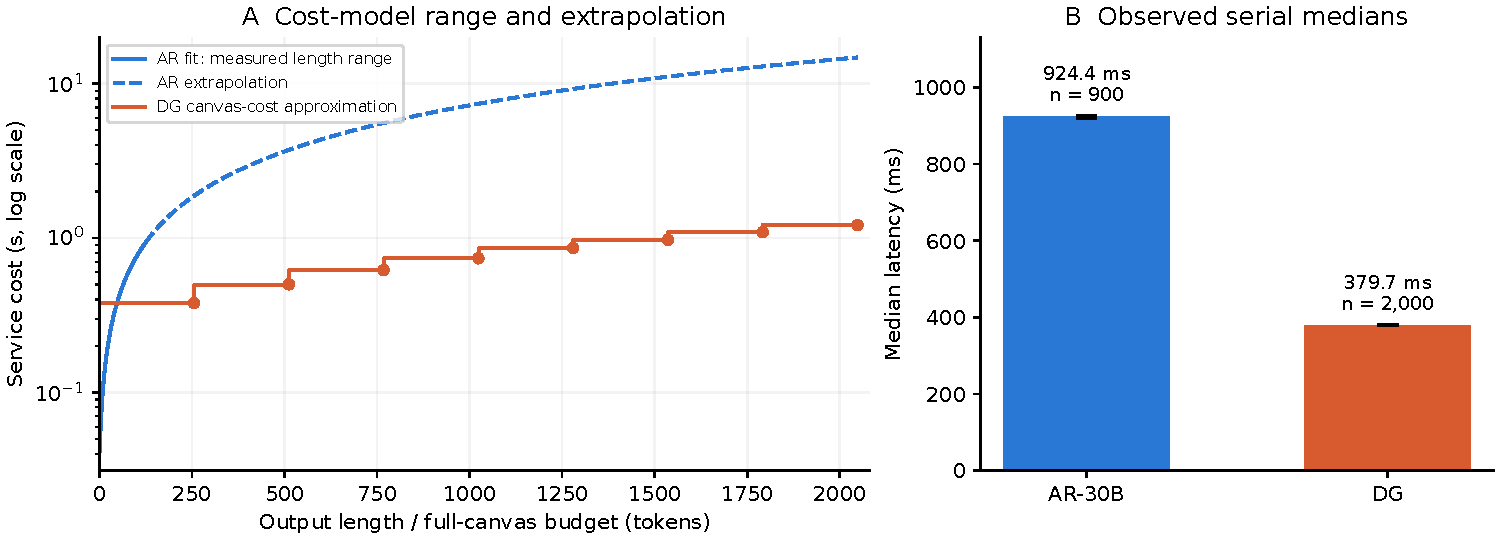
\includegraphics[width=\linewidth]{figures/fig1_v8.pdf}
\caption{Two distinct comparisons. Left: fitted cost versus generated output
length at a fixed reference prompt. The dashed AR continuation is an
extrapolation beyond the measured natural output length; DG points are
canvas-sweep measurements. Right: observed batch-1 median latency for the
main pair, with bootstrap 95\% intervals (AR: 900 events; DG: 2,000).
The left panel does not measure task-level speedup for long natural outputs.}
\label{fig:shapes}
\end{figure}

\section{Introduction}
\label{sec:intro}

Parallel token generation can shorten a language model's response time,
but it does not by itself establish a serving advantage. A useful comparison
must account for output length, stopping policy, concurrent requests, and
output quality. Autoregressive (AR) decoding generates tokens sequentially;
block-diffusion decoding refines a canvas of token positions in parallel
before moving to the next canvas. These execution patterns suggest different
latency curves. Their practical consequences require measurement.

We study structured log extraction on a single \gpuModel{} using
vLLM~\cite{vllm2023}. Our primary pair comprises
DiffusionGemma-26B-A4B (\DG)~\cite{diffusiongemma} and
Qwen3-30B-A3B (\ARthree)~\cite{qwen3}. Both are mixture-of-experts
(MoE) models with broadly comparable parameter and weight footprints.
This controls architecture class and approximate scale, but does not match
training data, model quality, tokenizer, or decoder implementation.
The main measurements use the pinned vLLM 0.25.1 stack. Earlier dense
Qwen2.5 and LLaDA experiments are identified separately throughout.

\paragraph{Task and data.}
Each raw log line is mapped to a JSON record with twelve fields. Seven
structural fields describe the timestamp, host, component, severity,
message template, error code, and numeric value; two fields encode an
anomaly label and score; three provide semantic or action information.
The primary corpus is BGL from LOGHUB~\cite{loghub}, containing
4{,}747{,}963 BlueGene/L log lines. The preparation procedure samples
600{,}000 lines by reservoir sampling (seed 42) and splits the sample
temporally into 400{,}000 training and 200{,}000 test records.
Evaluation cells use subsets of this test split, usually $n{=}300$ unless
otherwise stated. HDFS provides a secondary log-corpus check using the
2{,}000-line LOGHUB sample.

Reference records are constructed by the repository's parsing pipeline,
which supports Drain~\cite{drain} and a regex fallback. They are not
independently annotated semantic ground truth. In particular, the code
sets \texttt{is\_anomaly} when the native alert tag is non-normal
\emph{or} severity is ERROR, FATAL, or CRITICAL, and sets
\texttt{anomaly\_score} to the corresponding binary value. Thus these
fields measure agreement with a label-construction rule, not solely
prediction of native alert tags. A FATAL line tagged \texttt{-}, for
example, still receives an anomaly label under this rule.

\paragraph{Metrics and decoding.}
Quality is macro-averaged token-overlap F1 across seven structural and two
anomaly fields. We exclude \texttt{event\_type},
\texttt{affected\_entity}, and \texttt{remediation\_hint}, whose
references are parser-derived rather than independently validated.
Excluding them reduces one source of contamination; it does not make the
remaining labels independent of the preparation pipeline.
The scorer treats two empty field values as a match, so Field-F1 should be
read alongside validity. \emph{Schema validity} is the harness check for
required fields and supported type/enum constraints on the parsed record;
\emph{completeness} measures field presence. Neither establishes semantic
correctness. We use first-object-wins parsing for repeated JSON outputs.

Both models use greedy decoding (temperature 0, top-p 1, repetition
penalty 1). Unless varied explicitly, DG uses $K{=}8$ denoising steps
and canvas size $C{=}256$. Model-specific settings and environment versions
are recorded in the result artifacts. Nominal model sizes are 26B total/4B
active parameters for DG and 30B total/3B active for AR, with approximate
bf16 weight footprints of 52 and 60\,GB; these are rounded model labels,
not measurements of total runtime memory.

We distinguish three quantities: generated output length $L$, the configured
maximum output budget $B$, and the number of decoded canvases
$N_C$. Raising $B$ does not increase $L$ when a model has already emitted
end-of-sequence (EOS). We also distinguish serial mean service cost,
per-event latency percentiles, and inverse throughput under batching.
These quantities answer different deployment questions.

\paragraph{Contributions.}
\begin{itemize}
\item We fit an approximately linear AR cost model and a staircase DG cost
model, specifying the input-length, stopping-policy, and output-range
conditions under which they are useful (\S\ref{sec:laws}).
\item We measure a $2.4\times$ median-latency difference for the primary
pair at batch size one, and report the quality and statistical limitations
of that comparison (\S\ref{sec:wins}).
\item We quantify how batching, latency tails, prompt length, and decoding
effort change the deployment tradeoff (\S\ref{sec:limits}--\ref{sec:survives}).
\item We document nine groups of corrections to our own measurements and
interpretations, including defects that inflated the apparent diffusion
advantage (Appendix~\ref{app:defects}).
\end{itemize}

\begin{table}[ht]
\centering
\caption{Primary comparison. Latency statistics are from the repeated
BGL batch-1 runs (AR: 900 events; DG: 2,000). Throughput multipliers
come from separate batching experiments. DG has greater \emph{relative}
variability but lower \emph{absolute} p99 latency.}
\label{tab:summary}
\begin{tabularx}{\linewidth}{@{}L r r@{}}
\toprule
& \thead{AR-30B} & \thead{DG} \\
\midrule
\tabfont Nominal total / active parameters & 30B / 3B & 26B / 4B \\
\tabfont Approximate bf16 weights & 60\,GB & 52\,GB \\
\tabfont Median latency (ms) & \arMedian & \dgMedian \\
\tabfont p99 latency (ms) & \arPninetyNine & \dgPninetyNine \\
\tabfont Per-event CV (\%) & \arThirtyCV & \dgThirtyCV \\
\tabfont Observed batch-1 to peak multiplier & \arBatchMult$\times$ & up to 1.7$\times$ \\
\bottomrule
\end{tabularx}
\end{table}

\begin{table}[ht]
\centering
\caption{Simplified serial execution models at fixed prompt and decoding
settings. ``Flat'' refers to observed latency within a paid-for canvas,
not zero computation per token.}
\label{fig:schematic}
\begin{tabularx}{\linewidth}{@{}L L L@{}}
\toprule
& \thead{Autoregressive} & \thead{Block diffusion} \\
\midrule
Decoding & Sequential token steps & Parallel positions, sequential canvases \\
Cost approximation & $a_A+b_A L$ & $a_D+s_D(N_C-1)$ \\
Main variable & Actual generated length $L$ & Decoded canvas count $N_C$ \\
\bottomrule
\end{tabularx}
\end{table}

\section{Empirical cost models}
\label{sec:laws}

\subsection{Execution patterns and scope}
Standard AR decoding adds one token per decoding step, reusing the
request's existing key-value (KV) cache. Speculative decoding can change
this schedule and is not part of our primary baseline. DG refines token
positions jointly within a canvas and generates successive canvases
sequentially. Its encoder processes and caches context; its decoder
attends to that context while refining the active canvas~\cite{diffusiongemma}.
Revising canvas tokens can require recomputing their activations, but this
is distinct from recomputing the entire prompt.

The following models describe the measured implementation at batch size
one, a fixed reference prompt (approximately \refPrompt{} DG tokens),
$K{=}8$, and $C{=}\canvasLength$. They are empirical approximations,
not asymptotic laws valid for every runtime or input length:
\begin{align}
\label{eq:ar}
\widehat T_A(L) &= \arBase + \arSlope L && \text{ms},\\
\label{eq:dg}
\widehat T_D(N_C) &= \dgBase + \dgStep(N_C-1) && \text{ms},\qquad N_C\geq1.
\end{align}
For a full-budget canvas sweep, $N_C=\lceil B/C\rceil$. Substituting
$\lceil L/C\rceil$ is appropriate only when $L$ determines the number
of canvases actually decoded. EOS handling can make the budget and
emitted length different.

The AR fit uses cell mean service times and actual mean output lengths
from the serial sweep. Its five cells contain only three distinct
lengths, because three larger budgets stop at the same natural EOS.
The fit therefore supports the short-output range, roughly 32--126 tokens;
its longer continuation is an extrapolation. The DG base and canvas
increments summarize median-latency measurements. These different summary
statistics make their fitted intersection descriptive; the direct
median-to-median comparison appears in \S\ref{sec:wins}.
Neither fitted intercept isolates a physical operation such as prefill
without a separate timing breakdown.

\subsection{Crossover and canvas boundaries}
Within the first canvas, equating the two fitted costs gives
\begin{equation}
\label{eq:lcross}
L^* = \frac{\dgBase-\arBase}{\arSlope}\approx\crossoverL
\quad\text{tokens}.
\end{equation}
This is a cost crossover, not the minimum length at which a valid record
can be produced. It is conditional on the reference prompt and the two
fitted summaries. Beyond one canvas, the comparison must include the cost
of each additional canvas and the actual stopping policy. A larger budget
can increase DG's full-canvas cost while leaving AR's EOS-terminated cost
unchanged (Table~\ref{tab:niche}).

The reciprocal of the first-canvas median,
$1000/\dgBase\approx\crossoverLambda$ events/s, is a rough
serial service-rate scale. It is not a queueing threshold: capacity depends
on \emph{mean} service time and scheduling, and waiting can occur below
capacity under variable arrivals.

\begin{figure}[ht!]
\centering
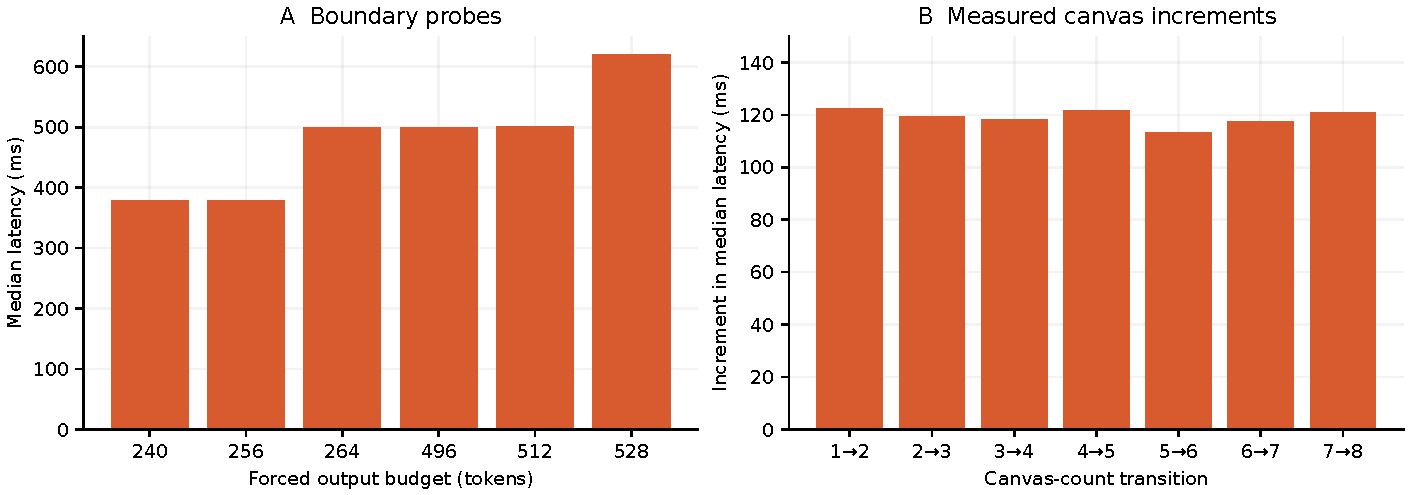
\includegraphics[width=\linewidth]{figures/fig2_canvas_edges.pdf}
\caption{DG canvas-boundary sweep ($K{=}8$, BGL, $n{=}200$ per cell).
Latency is approximately flat within each canvas and increases at the
boundary. The seven measured increments to $B{=}2048$ have median
\dgStep\,ms and range \dgStepLo--\dgStepHi\,ms. A constant
increment is a useful approximation within this sweep.}
\label{fig:edges}
\end{figure}

\subsection{Decoding effort and input dependence}
$K{=}8$ is a useful operating point in the tested quality--latency curve,
not a universal optimum. The $K$ sweep is nonlinear: measured latency
changes little from $K{=}8$ to $16$, then rises at $32$.
A line through the $K{=}2$ and $8$ observations gives an intercept near
143\,ms and a $K$-dependent contribution near 236\,ms at $K{=}8$.
This two-point interpolation does not identify prompt, attention, or
kernel costs, and cannot predict the benefit of a cache change
(Appendix~\ref{app:decomp}).

Longer prompts also increase latency. In the input-length experiment,
DG's fitted input slope is approximately \inputSlopeRatio$\times$
the dense AR-3B's. This is a secondary-model comparison, not an AR-30B
measurement. The dependence motivates the more general form
$T(L_{\mathrm{in}},N_C,K)$ and limits use of Eq.~\ref{eq:dg} when
schema width or conversational history changes
(Appendix~\ref{app:input_canvas}).

\paragraph{Transfer checks.}
At matched canvas size and $K$, the measured DG canvas increment changes
from \bglStep\,ms on BGL to \hdfsStep\,ms on the HDFS sample, a
1.7\% difference. This supports transfer of that increment between these
two settings. The AR slope comparison across corpora uses dense AR-3B.
For AR-30B, the HDFS median is \hdfsMedian\,ms (95\% bootstrap CI
[\hdfsCiLo, \hdfsCiHi]), with longer mean output than BGL; this
single operating point does not validate an entire cost curve.

HumanEval provides an exploratory task-transfer check
(Appendix~\ref{app:humaneval}). DG is faster in that harness but has
substantially lower pass@1 and syntax validity. Those measurements support
a latency--quality tradeoff, not a quality-matched code-generation speedup
or a demonstrated staircase across multiple code-output lengths.

\section{Serial latency, quality, and energy}
\label{sec:wins}

\paragraph{Direct latency comparison.}
In the repeated BGL runs at batch size one, AR-30B has median latency
\arMedian\,ms (95\% bootstrap CI [\arCiLo, \arCiHi]; 900 events
pooled across seeds 42, 137, and 314). DG has median \dgMedian\,ms
(CI [\dgCiLo, \dgCiHi]; 2,000 events). The ratio of these medians
is approximately $2.4\times$. Bootstrap intervals use 10,000 event-level
resamples. The AR seed-median CV is \seedCV\%, describing repeatability
across these three runs rather than uncertainty across hardware or workloads.

A two-sided permutation test of the absolute median difference observed
no equally or more extreme result in 100,000 shuffles. The finite-sample
Monte Carlo estimate $(0+1)/(100000+1)$ is approximately $10^{-5}$;
we do not interpret the stored zero exceedance fraction as a zero
probability. This unpaired test treats event timings as exchangeable and
does not control run-level differences or temporal dependence. The
observed latency gap is large, but its interval is conditional on these
measurement assumptions.

\begin{figure}[ht!]
\centering
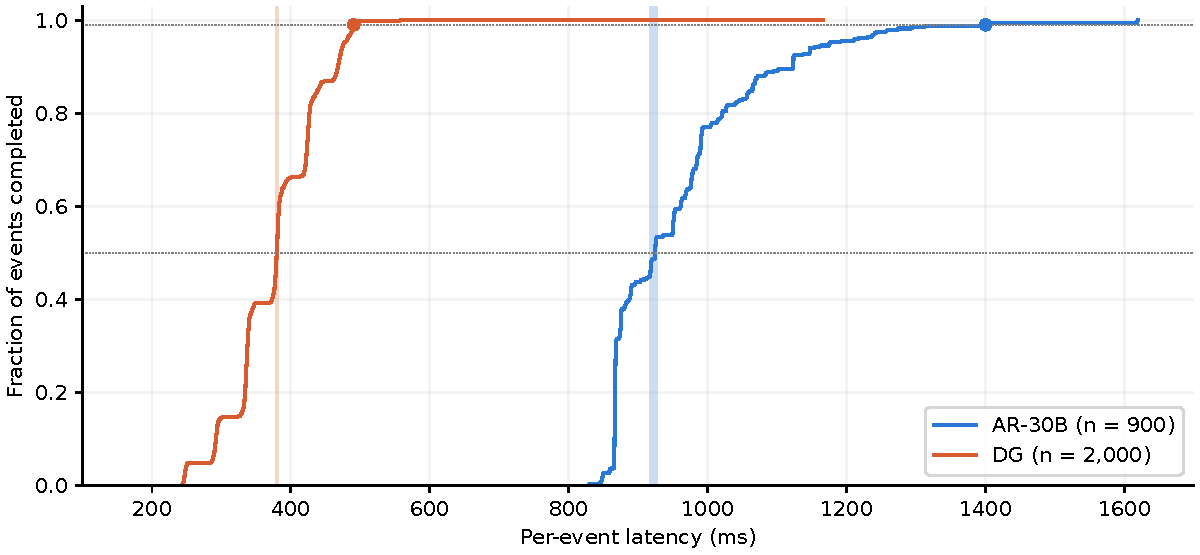
\includegraphics[width=0.88\linewidth]{figures/fig12_v8.pdf}
\caption{Empirical cumulative distributions of saved BGL event latencies:
AR-30B, 900 events across three seeds; DG, 2,000 events. Shaded bands
mark bootstrap 95\% intervals for each median. DG has lower median and
p99 latency, despite a larger coefficient of variation and max/median
ratio. These are service times, excluding arrival-queue delay.}
\label{fig:distributions}
\end{figure}

\paragraph{Quality is a separate constraint.}
The serial-sweep AR-30B 9-field F1 is 0.870. The earlier paired quality
analysis compared DG with dense AR-3B (\arThreeBFnine), not AR-30B.
It therefore cannot establish quality equivalence for the primary latency
pair. Faster service may be useful when DG meets the application's quality
threshold, but the current evidence does not establish a $2.4\times$
speedup at matched quality. This distinction also applies to the
throughput and cost comparisons.

\paragraph{Output budget is not generated length.}
Table~\ref{tab:niche} retains the original serial-sweep means so that
the fitted cost model can be traced to its source. These are different
runs and a different summary statistic from the repeated medians above.
AR emits approximately 126 tokens when its budget is sufficient and
then stops. Increasing the budget from 256 to 1024 does not lengthen
its output. By contrast, charging DG for all canvases permitted by the
budget increases its predicted cost. The resulting ratio is a
\emph{budget-accounting comparison}, not an observed long-output task
speedup.

\begin{table}[ht]
\centering
\caption{AR serial-sweep mean service time ($n{=}300$ per cell) versus
DG full-canvas cost from Eq.~\ref{eq:dg}. DG values are predictions
from measured canvas costs, not paired event means. The AR rows at
budgets 32 and 128 are output-limited; a 48-token cost crossover does
not imply valid extraction at that budget.}
\label{tab:niche}
\begin{tabular}{@{}rrrrr@{}}
\toprule
Budget $B$ & AR mean (ms) & AR mean tokens & DG model (ms) & AR/DG \\
\midrule
32 & 265 & 32 & 379 & $0.7\times$ \\
128 & 907 & 121 & 379 & $2.4\times$ \\
256 & 945 & 126 & 379 & $2.5\times$ \\
512 & 945 & 126 & 498 & $1.9\times$ \\
1024 & 945 & 126 & 737 & $1.3\times$ \\
\bottomrule
\end{tabular}
\end{table}

Extending this accounting to a 2048-token DG budget reverses the
ratio to approximately $0.8\times$: AR has already stopped while DG
is charged for eight canvases. Conversely, a task that actually requires
long AR output could widen DG's advantage. That case requires a new
natural-output evaluation; Appendix~\ref{app:forced} labels the
available calculation as a projection.

\paragraph{Throughput is not response latency.}
The AR-30B batch experiment completes 300 requests in 12.08\,s,
corresponding to 40.3\,ms per event when total elapsed time is divided
by batch size. Individual requests do not therefore return in 40.3\,ms.
That inverse-throughput measure must not be substituted for serial
response time. It underlies the approximately $25\times$ batching
multiplier in \S\ref{sec:limits}.

\paragraph{Energy.}
The saved AR-30B serial power run reports \arEnergy\,J per event
above idle, compared with \dgEnergy\,J for DG in a separate run.
The descriptive ratio is approximately $40\times$. The AR run records
223.0\,W mean board power, 49.73\,W idle, and 288.249\,s for 300
events; the DG run records 63.4\,W, 52.6\,W idle, and 38.57\,s for
100 events. Thus the direction is consistent with both lower DG net
power and shorter service time in these runs.

These measurements use different idle baselines, sample counts, and
power-sampling rates, with only 39 power samples in the DG run.
They do not isolate an architectural cause, and the idle-subtracted
ratio is sensitive to the small DG difference between active and idle
power. We treat it as preliminary board-energy evidence, not an
end-to-end energy-efficiency ratio or a controlled deployment-cost result.

\section{Deployment constraints}
\label{sec:limits}

\paragraph{Batching and concurrency.}
AR-30B improves throughput by \arBatchMult$\times$ in its batching
experiment, whereas DG reaches up to $1.7\times$ in the tested
configurations. LLaDA-8B on dInfer reaches approximately $1.2\times$.
The diffusion measurements are implementation-limited: the tested vLLM
path restricts mixed-phase batches, and dInfer was run without its
intended cache. They establish modest gains on those stacks, not an
upper bound on diffusion batching.

\begin{figure}[ht!]
\centering
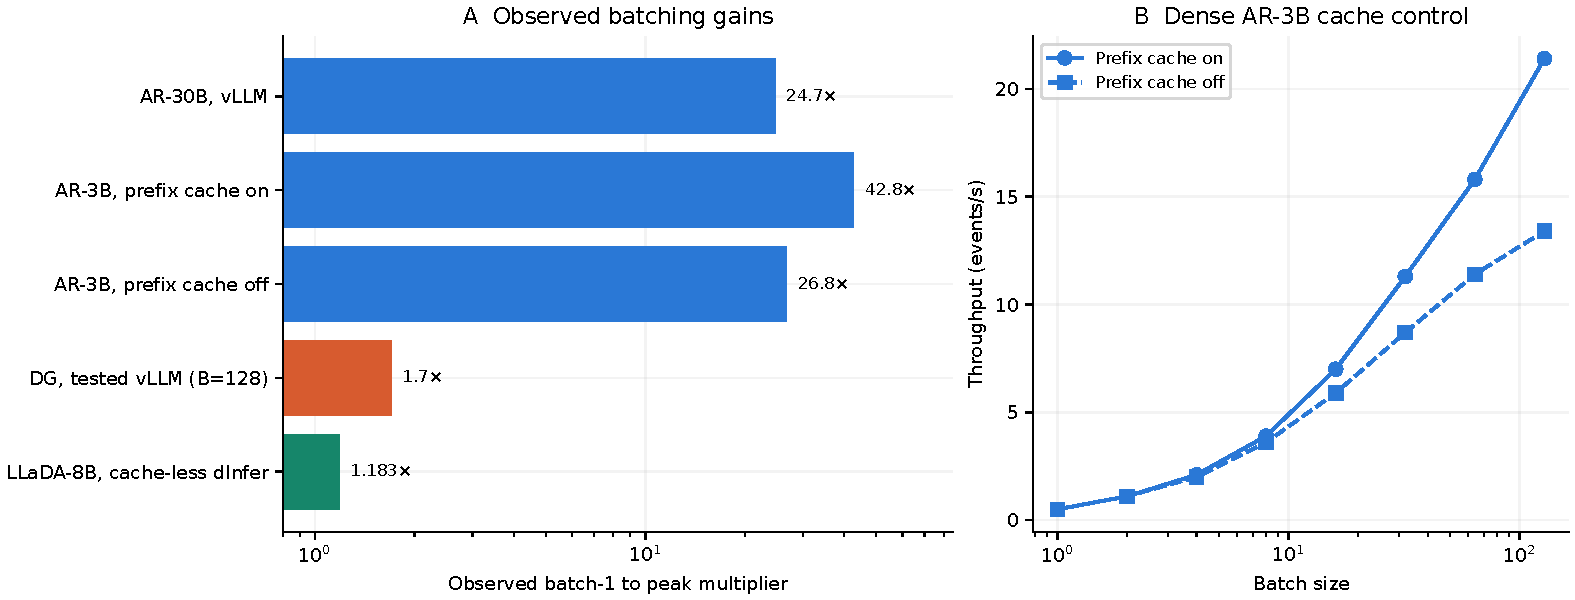
\includegraphics[width=\linewidth]{figures/fig6_batching.pdf}
\caption{Observed throughput multipliers for several model/runtime pairs.
The primary AR-30B result is approximately $25\times$. The cache-on/off
control uses dense AR-3B. Disabling cross-request
prefix caching lowers that model's multiplier from \cacheOnMult$\times$
to \cacheOffMult$\times$, so shared prefixes alone do not explain
its throughput gain. These controls do not identify a universal DG limit.}
\label{fig:batching}
\end{figure}

Sequential steps within one request chain cannot batch with each other,
but requests from independent chains can still overlap. Likewise,
interactivity and tenant isolation do not necessarily require a dedicated
batch-1 GPU. Deployment decisions should use measured arrival patterns,
scheduler behavior, and latency targets. Appendix~\ref{app:batching}
separates the cache observations from possible explanations.

\paragraph{Absolute and relative tails.}
In the repeated primary-pair measurements, AR-30B has CV
\arThirtyCV\% and max/median $1.75\times$, compared with
\dgThirtyCV\% and $3.07\times$ for DG. However, DG's absolute
p99 is \dgPninetyNine\,ms versus AR's \arPninetyNine\,ms.
A larger relative tail does not imply a slower absolute response or
an SLA violation. The relevant test is the specified latency percentile
under the intended arrival process. Sample maxima are not worst-case
bounds, and comparing maximum ratios across unequal sample sizes is
particularly fragile (Appendix~\ref{app:distributions}).

\paragraph{Prompt length and decoding settings.}
Longer prompts increase DG cost and can move the fitted crossover.
The input-slope comparison uses dense AR-3B and cannot be transferred
numerically to AR-30B. Canvas size and $K$ also change both cost and
quality. A joint sweep finds a better measured operating point than the
paper's reference setting: canvas 128, $K{=}8$ gives 368\,ms and
F1 0.864 versus 376\,ms and 0.853 at canvas 256, $K{=}8$.
These are point estimates on one sample, not a statistically established
improvement for all workloads (Appendix~\ref{app:input_canvas}).

\paragraph{Memory and co-residency.}
The nominal 52--60\,GB bf16 weight footprints of the primary pair
leave limited space for other large models on an 80\,GB GPU. Actual
capacity also depends on KV caches, activations, and runtime allocations.
A dense AR-1.5B has much smaller weights, but dividing GPU memory by
weight size cannot establish how many serving replicas fit or how their
throughput scales. We have not measured concurrent replicas, contention,
or isolation overhead, and make no linear co-residency speedup claim.

\paragraph{Cost accounting.}
At an assumed GPU rental rate $r$ dollars/hour, mean service time
$\bar t$ seconds/event, and busy fraction $u$, a simple single-instance
allocation is
\begin{equation}
 c_{\mathrm{event}}=\frac{r\bar t}{3600u}.
\end{equation}
This assumes the same GPU is rented throughout both busy and idle periods;
it excludes CPU, storage, networking, and retry costs. At fixed demand,
lower latency does not reduce the bill for an always-on GPU unless it
allows fewer provisioned resources or more useful work. A latency-based rental estimate therefore does not establish realized
annual savings. Batching economics should use measured throughput and
the quality requirement, rather than a serial latency ratio alone.

\section{Workloads and decoding-effort tradeoffs}
\label{sec:survives}

The measurements motivate a practical evaluation procedure rather than a
universal model-selection rule:
\begin{enumerate}
\item Measure natural output length and both models' stopping behavior;
check that the required record fits the chosen canvas budget.
\item Determine whether requests can overlap, including across independent
chains, and benchmark that concurrency on the intended serving stack.
\item Require both candidates to meet task-specific quality and schema
validity thresholds; a completed canvas is not a validated record.
\item Compare absolute latency percentiles, retries, and queueing delay
against the actual deadline or service-level agreement (SLA).
\item Include runtime memory, utilization, and energy at the chosen
canvas size and decoding effort.
\end{enumerate}

\paragraph{Serial investigation chains.}
An investigation can require dependent steps: inspect an alert, retrieve
context, and choose a follow-up query. This makes serial model latency
relevant within a chain. The BGL chain harness compares DG with dense
AR-3B, at approximately 419 and 808\,ms per hop, respectively.
It does not directly measure an AR-30B chain or the retrieval and tool
latencies of a deployed investigation system.

\begin{figure}[ht!]
\centering
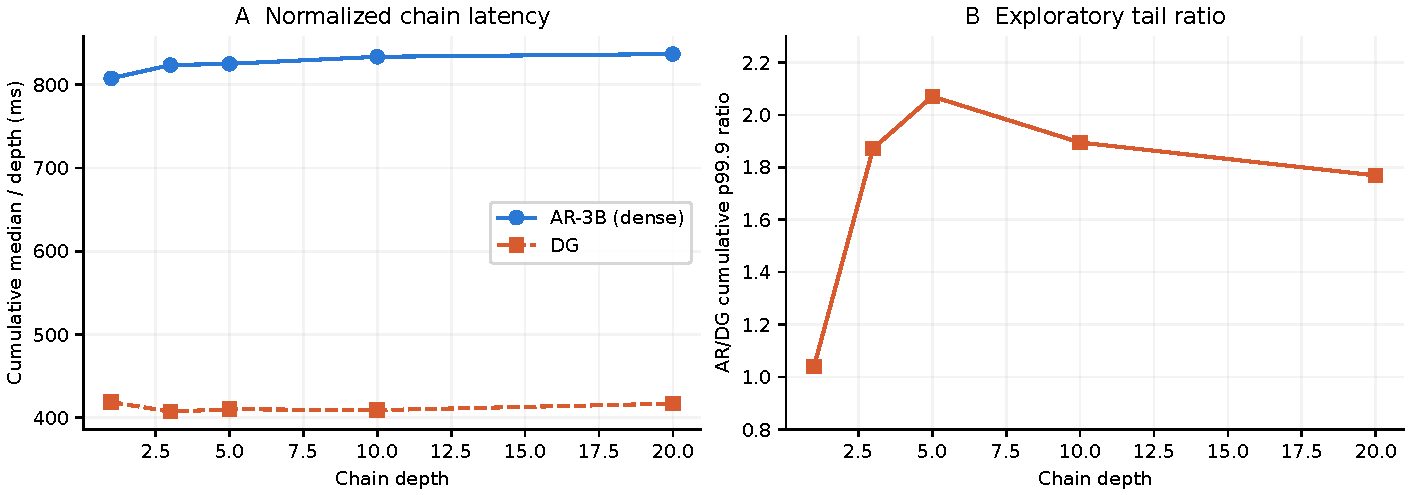
\includegraphics[width=\linewidth]{figures/fig10_usecase_chains.pdf}
\caption{BGL chain-harness latency (DG versus dense AR-3B; $n{=}100$
chains per depth, $K{=}8$). Cumulative median cost divided by depth is approximately constant
in this experiment. The cumulative tail ratio varies with depth.
With only 100 chains, the plotted p99.9 is effectively an extreme-order
statistic and should not be used to certify a production tail target.}
\label{fig:chains}
\end{figure}

The latency gap accumulates when several dependent calls are required,
but neither the quality of a complete investigation nor independence of
hop latencies follows from this curve. The HumanEval correction-chain
artifact reports total-chain and first-round medians; those are not
per-round latency growth rates (Appendix~\ref{app:humaneval}).

\paragraph{Reducing effort before a deadline.}
DG exposes a denoising-effort control, $K$. In the BGL sweep, reducing
$K$ from 8 to 4 lowers quality from \kEightFone{} to \kFourFone{}
while yielding p99 \kFourPninetynine\,ms. This operating point
falls below a 400\,ms service-time budget in that sample. It does not
guarantee valid JSON, completion under arbitrary interruption, or a
400\,ms end-to-end deadline. Selecting a lower $K$ before generation
is different from safely preempting an unfinished canvas.

Under an output-length cap of 128 tokens, DG's schema validity falls to
\dgValidTwentyEight\%, compared with \arValidTwentyEight\% for
dense AR-3B. Thus lowering denoising effort and shortening the output
budget have different effects (Appendix~\ref{app:quality}). AR also
admits adaptive budgets, early stopping, retries, and routing policies;
we do not claim that adaptive computation is unique to diffusion.
Grammar-constrained AR remains an important unmeasured comparator.

\paragraph{Wide schemas.}
Across schemas with 12--100 fields, DG's measured latency advantage
against dense AR-3B ranges from approximately $1.8\times$ to
$3.0\times$. Both prompt and output lengths change, and the models
emit different token counts. This is a useful workload comparison,
but does not isolate a benefit from joint inter-field reasoning.
The consistency evaluator checks three fixed rules over four fields at
every width, so it cannot establish scaling with the number of
pairwise constraints.

\begin{figure}[ht!]
\centering
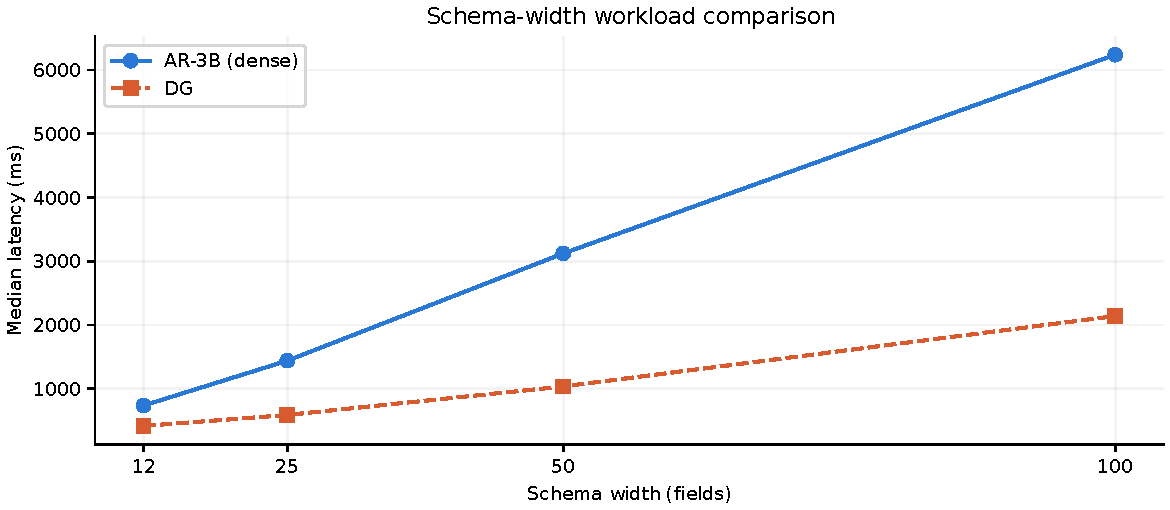
\includegraphics[width=0.85\linewidth]{figures/fig11_usecase_schema.pdf}
\caption{Latency versus schema width (BGL, $n{=}200$; dense AR-3B
baseline). DG's advantage rises from about $1.8\times$ to
$2.9$--$3.0\times$. Input length, output length, and canvas count
change together, preventing a causal attribution to schema width alone.}
\label{fig:schema}
\end{figure}

\paragraph{Adaptive effort: a measured negative result.}
A two-stage cascade first runs DG at $K{=}2$, checks structural-field
completeness, and reruns unresolved inputs at $K{=}8$. In the BGL
experiment ($n{=}200$), 29.5\% of records finish at the first stage
and 70.5\% escalate. F1 is 0.848 versus 0.853 for fixed $K{=}8$;
mean latency increases to 465\,ms from 376\,ms. The extra low-effort
pass costs more than it saves. Completeness is also only a proxy for
correctness. A lower escalation rate could improve this tradeoff, but
that benefit is not observed here.

\paragraph{Scope of application claims.}
The evidence concerns log extraction and exploratory code-generation
harnesses. We have not evaluated driving, trading, or deployed security
response, and do not infer suitability for those applications from
batch size or latency shape. Even in logs, the deployment choice depends
on quality, output validity, arrival rate, and the available AR baseline.
Appendix~\ref{app:refuted} reports the hypotheses that were contradicted
or left unsupported by the experiments.

\section{Related work}
\label{sec:related}

LLaDA~\cite{llada2025} studies language modeling through masked
diffusion. DiffusionGemma~\cite{diffusiongemma} combines block-wise
diffusion with an encoder that caches context. Our contribution is an
empirical comparison of serving behavior for particular public models,
with explicit output-budget, latency-statistic, and quality constraints.
We do not claim that linear and staircase execution patterns are new,
or that these measurements isolate architecture from implementation.
PagedAttention and vLLM~\cite{vllm2023} provide the serving foundation;
using the same engine version removes one source of comparison bias,
but does not make its model-specific execution paths identical.

Grammar-constrained generation, including Outlines~\cite{outlines2024},
XGrammar~\cite{xgrammar2024}, and llguidance~\cite{llguidance},
addresses structured-output validity through token constraints.
This is complementary to choosing a decoding schedule. A completed
sampling run and an output that satisfies a grammar are different
properties; our unconstrained comparison cannot settle their joint
latency--quality tradeoff.

Speculative methods such as Medusa~\cite{medusa2024} and
EAGLE~\cite{eagle2024} verify multiple proposed tokens per iteration.
Their effective cost depends on acceptance, verification, and workload;
they need not obey the fitted slope of our standard AR baseline.
Our older n-gram prompt-lookup experiment on dense AR-3B is not a
comparison against those methods or a bound on optimized AR inference.
A tuned speculative AR-30B baseline is a useful next comparison.

Hoefler and Belli~\cite{hoefler2015} discuss experimental design and
reporting in systems benchmarking. The corrections in
Appendix~\ref{app:defects} provide a case study of how decoding
defaults, parsers, labels, and timing conventions affect a model-serving
comparison. They motivate explicit provenance and artifact checks,
without supporting an allegation about other authors' intentions.

\section{Limitations and reproducibility}
\label{sec:threats}

\paragraph{Scope and model matching.}
The primary comparison uses one DG checkpoint and one AR checkpoint on
one A100 80GB. Similar MoE scale does not control training, tokenizer,
quality, or implementation. The fitted constants are specific to the
measured stack, prompts, and decoding settings. Dense AR-3B and
LLaDA results support narrower secondary observations; they must not be
silently substituted for the primary pair. HDFS and HumanEval extend
the coverage but do not establish generalization across deployment tasks.

\paragraph{Quality and reference construction.}
The reported quality-equivalence interval is for DG versus dense AR-3B:
the 95\% interval for the paired difference is $[-0.012,+0.011]$
at $n{=}300$. It fits within a $\pm0.015$ margin, but not the
originally targeted $\pm0.010$ margin; the latter holds only for the
reported 90\% interval. Widening the margin after observing results
must not be described as confirmation of the original criterion.
No corresponding equivalence test establishes quality matching for
AR-30B. Reference labels are parser-derived, and the anomaly rule also
uses severity. The metric therefore measures a restricted extraction
objective, not independently assessed semantic or anomaly-detection quality.

\paragraph{Output range and uncertainty.}
The AR cost fit has five budget cells but only three distinct actual
output lengths, concentrated near 32 and 126 tokens. Its high fit score
cannot validate extrapolation to thousand-token natural output.
DG's longer canvas sweep also holds the reference task and prompt fixed.
A task with naturally longer output may require more input and produce
a different quality--latency tradeoff. The cost intersection also combines
AR cell means with DG median summaries.

The main latency bootstrap resamples events, not independent machines or
complete experimental runs. Only AR has the three-seed timing comparison;
we do not claim multi-seed replication of both arms. Shared prompts,
cache warm-up, or time-correlated timings can violate independent-event
assumptions. The permutation comparison is unpaired and does not eliminate
run-level confounding. Extreme quantiles remain uncertain: p99.9 uses very
few observations even with 900 AR and 2,000 DG events. A sample maximum
is not a service-time bound.

\paragraph{Serving mechanisms and comparators.}
Both diffusion batching measurements have engine limitations. The
model's documented context cache contradicts a blanket claim that diffusion
cannot reuse KV state. Neither the batching control nor the two-point
$K$ interpolation isolates a universal architectural bottleneck.
A hardware profile and an optimized cache-enabled control are needed for
such attribution (Appendix~\ref{app:batching_architectural}).

A tuned grammar-constrained AR comparison has not been completed on the
pinned stack. An older outlines-backed AR-1.5B experiment on vLLM 0.10.2
returned only 1.0\% valid records and cannot bound what a current tuned
configuration can achieve. Grammar constraints can improve validity, but
do not guarantee completion under arbitrary time or token limits.
Modern speculative decoding is also outside the primary comparison.

\paragraph{Secondary results.}
The energy measurements have different idle baselines and sampling rates,
so their ratio is descriptive. Replica co-residency and realized rental
savings were not measured. Wide-schema consistency uses only three fixed
rules. Chain-tail estimates use 100 chains per depth. HumanEval's
single-pass and correction-chain artifacts have substantially different
first-round scores; those must be reconciled before treating them as
replication of the same task protocol. The deadline experiment maps time
to token budgets rather than enforcing a wall-clock cutoff
(Appendix~\ref{app:humaneval}).

\paragraph{Reproducibility.}
Code and committed results are available at
\href{https://github.com/AlexKay28/DLLM-as-Service}{the DLLM-as-Service repository}.
The primary stack is vLLM 0.25.1, torch 2.11.0, and CUDA 13.0 on an
A100 80GB. Experiment entry points are in
\texttt{models/experiments/}; model, parser, and stack settings should be
read from each artifact's provenance, since historical campaigns differ.
\texttt{analysis/ar30b\_stats.py} identifies the per-event files used
for the primary statistical comparison. The repository verifier checks
selected macro-to-artifact mappings and provenance; it does not certify
every prose number, experimental assumption, or source citation.
The manuscript snapshot includes a separate numeric audit and build instructions.

Compute use is estimated at approximately 20 GPU-hours for reported
experiments and 10 additional hours for preliminary and failed runs.
These are author estimates, not a reconstructed usage ledger. Token counts are
reported as workload descriptors, not a hardware-normalized FLOP measure.
The models, datasets, and libraries retain their respective upstream
licenses; the relevant source locations are cited. Revision-specific
license records should accompany a release of the experiment environment.

\paragraph{Broader impact and assisted editing.}
More efficient inference could reduce resources needed for structured
extraction, but validity and accuracy remain necessary for any downstream
action. These measurements do not validate safety-critical deployment.
The study uses public models and datasets and involves no human subjects.
An LLM-based assistant supported editorial review, claim checking,
and document preparation.

\section{Conclusion}
\label{sec:conclusion}

For the measured BGL extraction workload, DiffusionGemma provides lower
batch-1 latency than Qwen3-30B-A3B on the same pinned serving stack:
approximately 380 versus 924\,ms at the median. AR throughput benefits
much more from batching in the tested configurations. The resulting
tradeoff depends on the workload's concurrency and quality requirements.

A linear AR cost approximation and a DG canvas staircase help explain
these observations when their input and stopping conditions are explicit.
They do not establish a universal long-output speedup, a diffusion
batching ceiling, or guaranteed valid output under interruption.
Generated length must be separated from output budget, service latency
from inverse throughput, and statistical uncertainty from model quality.
The immediate practical use is to evaluate block diffusion for serial
structured extraction while validating the complete record and the
absolute latency tail on the intended workload. Quality-matched AR-30B,
tuned constrained or speculative AR, and naturally long-output tasks
remain the most consequential comparisons to complete.


% ======================================================================
%                          APPENDICES
% ======================================================================

\bibliographystyle{plain}
\bibliography{assets/references}

\appendix

\section{Corrections to the comparison}
\label{app:defects}

The study underwent nine groups of corrections. Several contain more than
one implementation defect, so this count is an audit organization rather
than a count of independent failures. Inspection of committed artifacts
identified the problems; some corrections required new measurements.
The effects below concern our own harness and should not be generalized
to other authors' experiments or intentions.

\begin{enumerate}
\item \textbf{Decoding configuration.} A checkpoint repetition penalty
suppressed span-copying. Setting it to 1.0 moved dense AR-1.5B's
12-field F1 from \defectOneFBefore{} to \defectOneFAfter{}
($n{=}2000$). The default had understated AR quality.
\item \textbf{Serving path.} Moving dense AR-1.5B from a HuggingFace
\texttt{generate} loop to vLLM changed p50 from
\defectTwoBefore{} to \defectTwoAfter\,ms ($n{=}2000$).
The earlier diffusion comparison therefore depended strongly on the AR
implementation. This historical comparison is not the current MoE pair.
\item \textbf{Parser policy.} At output budget 512, \rambleRate\%
of AR outputs contained multiple JSON objects. Taking the first object
rather than the last changed dense AR-3B's 12-field F1 from
\defectThreeBefore{} to \defectThreeAfter{}.
\item \textbf{Completeness.} A metric counted present but falsy values
such as \texttt{False}, \texttt{0.0}, and empty strings as missing.
Correcting field-presence handling changed the reported AR completeness
from \defectFourBefore\% to \defectFourAfter\% in the historical
bounded-deadline experiment, removing the claimed completeness advantage.
\item \textbf{Model provenance.} A CLI default wrote an AR identifier
into three LLaDA artifacts. Correction sidecars document the model used.
The error affected auditability rather than the stored timings.
\item \textbf{Classical baseline.} A result labeled ``Drain'' used a
regex fallback shared with reference construction. Self-agreement on
parser-derived fields was not an independent extraction benchmark;
we withdrew that comparison.
\item \textbf{Semantic references.} Three fields had parser-derived or
constant references. On the historical DG/dense-AR-3B pair, excluding
them changed the reported gap from \twelveGap{} on twelve fields to
approximately \qualityGap{} on nine. This does not remove all
reference-construction limitations (\S\ref{sec:threats}).
\item \textbf{Queueing interpretation.} A Poisson-arrival saturation
observation was overinterpreted as validation of an M/D/1 latency model.
The claim did not transfer to the bursty arrival experiment. We retain
the observed load behavior without a general queue-delay guarantee.
\item \textbf{AR-30B input and timing.} A historical harness supplied
gold records instead of raw logs, combined an older engine with eager
execution, mislabeled batched cost as serial latency, and mishandled
prediction construction. Its perfect quality and 48\,ms/token estimate
were invalid. Corrected measurements on the pinned stack gave
approximately 7.2\,ms/token and 9-field F1 0.870. The headline comparison
must use those corrected artifacts or the later repeated latency runs.
\end{enumerate}

The practical checks are explicit decoding settings, inspection of raw
inputs and outputs, separate timing and throughput definitions, and
verification of model identifiers and reference construction. A numeric
verifier can detect some transcription errors; it cannot establish that
a valid-looking metric measures the intended task.

\section{What the denoising-step sweep identifies}
\label{app:decomp}

The sweep $K\in\{2,4,8,16,32,64\}$ is poorly described by one line:
$T(K)=\kfitBase+\kfitSlope K$ has $R^2=\kfitRsq$.
Measured p50 is 378.6\,ms at $K{=}8$, 382.5\,ms at $16$,
421.8\,ms at $32$, and 423.9\,ms at $64$. This nonlinearity makes
extrapolation of a single intercept unreliable.

A line through $T(2)=201.7$\,ms and $T(8)=378.6$\,ms has an
intercept of approximately 142.7\,ms and a $K$-dependent contribution
of approximately 236\,ms at $K{=}8$. The decomposition is algebraic:
two points determine two coefficients. It is not a profiler measurement,
a validated zero-step latency floor, or a separation of prefill from
denoising work. In particular, it does not establish that a cache change
would remove 62\% of service time. The artifact named
\texttt{issue70\_profiler\_attribution.json} explicitly identifies
its method as analytical attribution, not a hardware profile.

\begin{figure}[ht!]
\centering
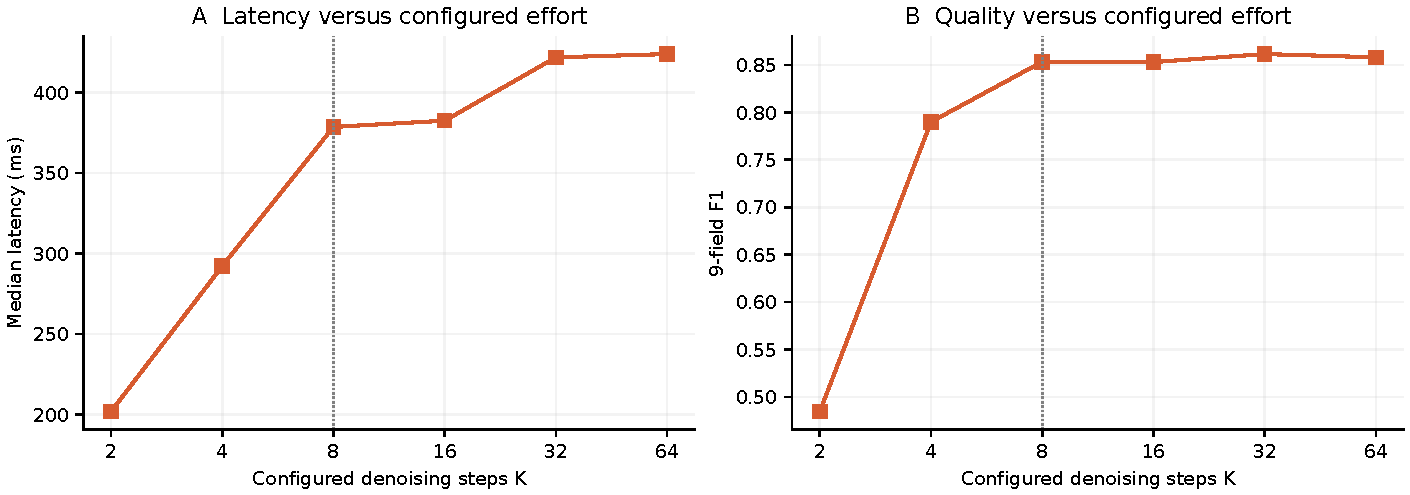
\includegraphics[width=0.85\linewidth]{figures/fig4_ksweep.pdf}
\caption{DG denoising-step sweep (BGL, $n{=}200$, output budget
\canvasLength). Latency is nonlinear in configured $K$. The observed
quality gains become small around $K{=}8$ in this sweep; that is a
practical operating-point choice, not a universal saturation threshold.}
\label{fig:ksweep}
\end{figure}

\section{Batching measurements and cache controls}
\label{app:batching}

The primary AR-30B batch run processes 300 events in 12.08\,s and
reports a throughput multiplier of \arBatchMult$\times$ relative
to its serial control. DG on vLLM reaches up to
\dgBatchVllmHi$\times$ in the tested length and batch settings;
LLaDA-8B on dInfer reaches approximately $1.2\times$.
The vLLM mixed-phase limitation and cache-less dInfer configuration
prevent either diffusion result from establishing an architectural ceiling.

The prefix-cache toggle is a separate dense AR-3B experiment. Turning
cross-request prefix caching off changes its multiplier from
\cacheOnMult$\times$ to \cacheOffMult$\times$.
This shows that shared-prefix reuse is not the sole source of AR's
batching gain. It does not isolate the remainder as within-request KV
persistence: kernel efficiency, weight reuse, scheduling, and batch shape
also differ. Appendix~\ref{app:batching_architectural} describes the
architectural distinction without assigning an unmeasured causal share.

\section{Negative and unsupported hypotheses}
\label{app:refuted}

The following hypotheses were contradicted by measurements, explained by
harness corrections, or not tested by the chosen metric. These are different
evidential outcomes. In particular, failure to measure a proposed scaling
law is not an empirical refutation of that law.

\begin{table}[ht]
\centering
\caption{Limits of proposed diffusion advantages on BGL. Perturbation,
refinement, and the historical deadline probe use LLaDA versus dense
AR-3B; infilling uses DG versus dense AR-3B; schema-width and output-budget
probes use DG with dense AR-3B controls. These are not AR-30B results.}
\label{tab:refuted}
\begin{tabularx}{\linewidth}{@{}>{\raggedright\arraybackslash}p{4.2cm}L@{}}
\toprule
\thead{Hypothesis} & \thead{Evidence and interpretation} \\
\midrule
\tabfont Greater perturbation robustness & \tabfont LLaDA degrades more than AR in all ten tested categories. This does not isolate bidirectional attention as the cause. \\
\tabfont Better infilling & \tabfont AR scores 0.993--0.999 across tested suffix sizes; DG falls from about 0.960 to 0.753 at eight held-out suffix tokens. This task permits AR to regenerate the record from its prompt. \\
\tabfont Refinement closes the quality gap & \tabfont LLaDA gains 0.023 F1 over three rounds but still trails one AR pass. The improvement does not establish a quality win. \\
\tabfont Guaranteed deadline completeness & \tabfont The historical AR completeness deficit disappeared after correcting treatment of falsy values (Appendix~\ref{app:defects}, item 4). \\
\tabfont Joint denoising absorbs quadratic constraint cost & \tabfont Not tested: the consistency metric checks three fixed rules at every schema width. \\
\tabfont Quality invariant to output budget & \tabfont DG quality is poor at small budgets, then rises and plateaus. A plateau over sufficient budgets is not global invariance. \\
\bottomrule
\end{tabularx}
\end{table}

These outcomes constrain the application claims. They do not establish
that diffusion is intrinsically less robust, incapable of infilling, or
unable to benefit from refinement. The measured model, task framing,
references, and decoding configuration remain part of each comparison.

\section{Input length and canvas tuning}
\label{app:input_canvas}

\subsection{Input length}
The input-length sweep repeats the schema block while holding the
extraction target fixed. DG's fitted input slope is approximately
\inputSlopeRatio$\times$ that of dense AR-3B. This demonstrates
input dependence in the tested paths. It does not imply that DG
recomputes all prompt KV state at every denoising step, nor does it
supply an input slope for AR-30B.

\begin{figure}[ht!]
\centering
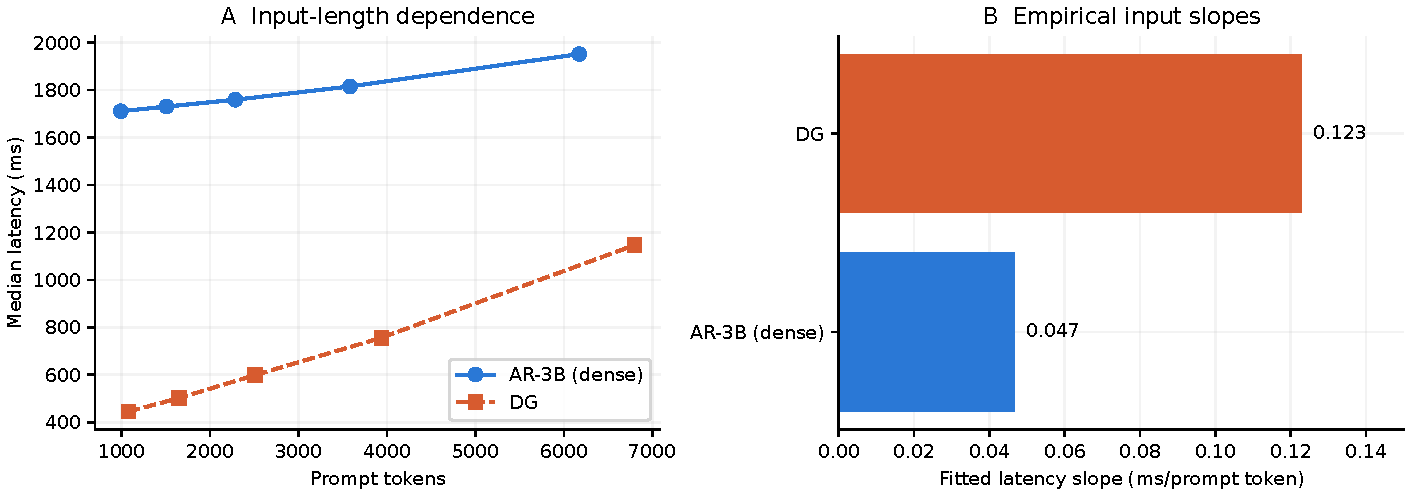
\includegraphics[width=\linewidth]{figures/fig3_input_sweep.pdf}
\caption{Input-length sweep at fixed output budget \canvasLength{}
(BGL, $n{=}100$ per cell; dense AR-3B baseline). Repeating the schema
changes the prompt length and redundancy together. Fitted slopes are
specific to this construction.}
\label{fig:input}
\end{figure}

\subsection{Canvas size and effort}
In the single-parameter sweep, canvas 128 yields median latency
\canvasOneTwentyEightBase\,ms and 9-field F1
\canvasOneTwentyEightFone{}. The joint sweep over canvas sizes
$\{64,128,256,512\}$ and $K\in\{2,4,8,16,32\}$ uses
$n{=}200$ per cell. At $K{=}8$, canvas 128 has observed p50
368\,ms and F1 0.864, compared with 376\,ms and 0.853 for canvas
256. It therefore dominates the reference setting in these two point
estimates. This is an empirical Pareto comparison over the tested grid,
not proof of a global optimum or a statistically established improvement.

Canvas 64 performs worse in the reported setting, but this does not make
it unusable for other output distributions. The reference setting remains
canvas 256, $K{=}8$ for continuity with the principal sweeps. Selecting a
new operating point should include uncertainty, valid-output rates, and
held-out workload evaluation rather than optimization on the same sample.
The joint data are in \texttt{results/issue114\_joint\_sweep.json}.

\section{Quality versus output budget}
\label{app:quality}

At output budget 128, dense AR-3B retains
\arFOneTwentyEight{} 9-field F1 and \arValidTwentyEight\%
schema validity, while DG has \dgFOneTwentyEight{} and
\dgValidTwentyEight\%. Thus a small budget can prevent usable DG
records even when the cost model predicts low latency. This experiment
varies the allowed output budget, not the native canvas-size setting.

\begin{figure}[ht!]
\centering
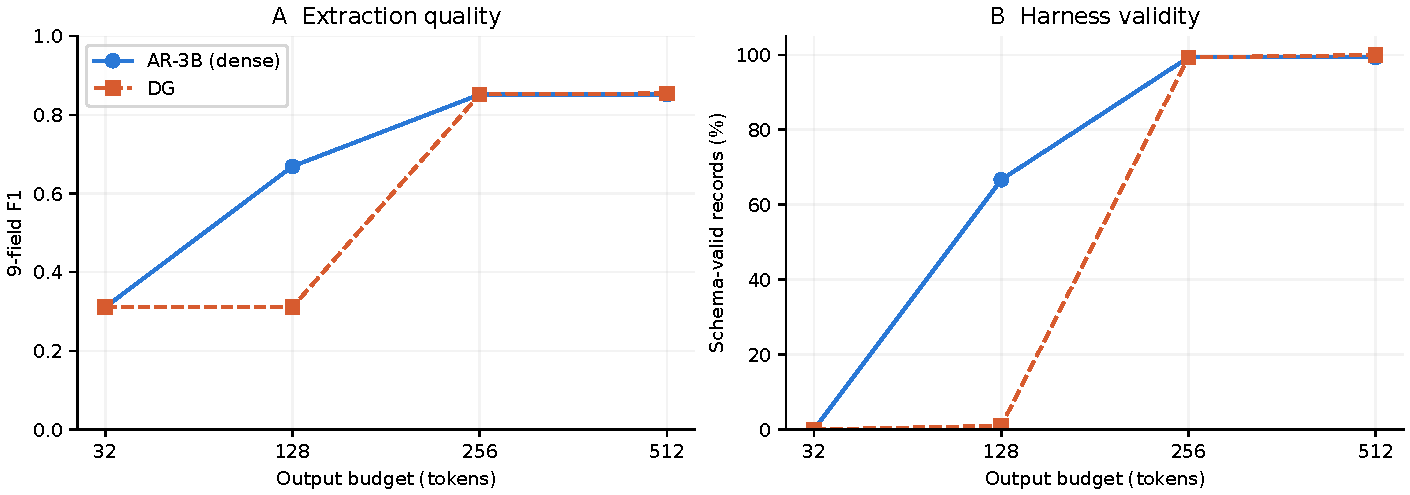
\includegraphics[width=\linewidth]{figures/fig5_quality_vs_length.pdf}
\caption{Quality and schema validity versus constrained output budget
(BGL, $n{=}300$; dense AR-3B baseline). DG improves sharply once the
budget permits a complete record. First-object-wins parsing keeps AR-3B
F1 stable from budgets 256 to 512 despite repeated continuations.
Neither curve constitutes a guarantee of valid output.}
\label{fig:quality}
\end{figure}

Lowering $K$ is a distinct intervention and can trade quality for service
time without reducing the nominal token budget. Its value must still be
assessed using observed validity and correctness; a denoised token canvas
can contain malformed or incorrect JSON.

\section{Latency distributions and tail interpretation}
\label{app:distributions}

The repeated primary-pair statistics are:
\begin{center}
\begin{tabular}{@{}lrr@{}}
\toprule
Statistic & AR-30B & DG \\
\midrule
Events & 900 & 2,000 \\
Median (ms) & \arMedian & \dgMedian \\
p99 (ms) & \arPninetyNine & \dgPninetyNine \\
p99.9 (ms) & 1619.1 & 557.0 \\
Maximum (ms) & 1619.2 & 1166.4 \\
CV (\%) & \arThirtyCV & \dgThirtyCV \\
\bottomrule
\end{tabular}
\end{center}

DG has greater relative variability, but lower absolute latency at all
listed quantiles. Inferring a failed SLA from its max/median ratio alone
would reverse the relevant comparison. With only 900 AR events, p99.9
is nearly the sample maximum; even DG's 2,000-event estimate represents
only a few tail observations. These measurements neither bound unseen
outliers nor include waiting under an arrival process. The event-level
bootstrap and permutation procedure are described in \S\ref{sec:wins};
the saved summary is \texttt{results/anchors/ar30b\_stats.json}.

\section{Projection for naturally longer output}
\label{app:forced}

The main budget table leaves AR near its natural EOS at 126 tokens
while charging DG for a specified number of full canvases. A different
question is whether a task that requires multiple records would make both
models generate longer outputs. Table~\ref{tab:forced} evaluates the
fitted equations at assumed output lengths for that scenario.

\begin{table}[ht]
\centering
\caption{Illustrative fixed-prompt cost-model extrapolation. Only the
single-record anchor is observed (AR mean versus DG median anchor).
Multi-record lengths and costs are assumed/calculated, not measurements
of multi-record extraction. Quality is not evaluated for those rows.}
\label{tab:forced}
\begin{tabular}{@{}lrrrr@{}}
\toprule
Scenario & Assumed $L$ & AR (ms) & DG (ms) & AR/DG \\
\midrule
Single-record anchor & 126 & 945 & 379 & $2.5\times$ \\
Two records & 280 & 2051 & 498 & $4.1\times$ \\
Four records & 560 & 4067 & 618 & $6.6\times$ \\
Eight records & 1120 & 8099 & 857 & $9.5\times$ \\
\bottomrule
\end{tabular}
\end{table}

The calculation assumes about 140 tokens per record and leaves the
reference prompt cost fixed. A real multi-record task also lengthens the
input and may change formatting, stopping behavior, and accuracy.
Consequently these ratios are hypotheses for a new experiment, not
validated speedups or evidence that the observed serial ratio is a
conservative lower bound.

\section{Cache reuse and possible batching mechanisms}
\label{app:batching_architectural}

Two different forms of cache reuse matter: sharing unchanged context
across requests, and preserving activations within a request as generation
progresses. In AR decoding, causal attention allows the already-generated
prefix's KV state to persist while new tokens are appended. During
bidirectional denoising, changing canvas tokens can invalidate activations
within that canvas. This can increase the work per refinement step.

It does not follow that diffusion must discard all cached context.
DiffusionGemma's documented encoder--decoder design caches the prompt and
completed canvases, while the active canvas uses bidirectional attention
and accesses encoded context~\cite{diffusiongemma}. A changing canvas
also does not require a changing attention mask at every step.

The observations are therefore compatible with several explanations for
modest batching gains: larger per-request kernels, different weight and
activation reuse, scheduling restrictions, and implementation-specific
cache behavior. The existing controls do not distinguish their shares.
We do not predict a maximum batching multiplier or claim compute
saturation at batch size one. Establishing such a mechanism would require
hardware profiling and matched cache/scheduling ablations on a working
optimized diffusion path.

\section{Cost-shape generalisation: code generation on HumanEval}
\label{app:humaneval}

The following exploratory measurements use HumanEval~\cite{humaneval}
(164 Python function-completion problems). They extend the workload
coverage but expose substantial quality and protocol limitations. Pass@1
is the fraction of first completions passing the harness tests; code
validity is the fraction accepted by Python syntax parsing. Neither is
guaranteed by completing a token canvas.

\subsection{Single-pass latency and quality}

Both arms were run serial (batch-1) on the pinned stack
(\S\ref{sec:threats}), $n{=}164$ problems.

\begin{table}[h]
\centering
\caption{Single-pass HumanEval results (serial, $n{=}164$). DG is
faster but has much lower pass@1 and syntax validity. The ms/token column
is median latency divided by mean generated tokens, not a fitted decode
slope. This table does not measure a cost curve across output lengths.}
\label{tab:humaneval}
\begin{tabular}{@{}lrrrrr@{}}
\toprule
Arm & pass@1 & code valid\% & p50 (ms) & mean tokens & ms/token \\
\midrule
DG K=8  & 0.287 & 31.1 & 280 & 99.5  & --- (staircase) \\
AR-30B  & 0.720 & 93.9 & 800 & 124.1 & 6.4 \\
AR-3B   & 0.573 & 99.4 & 560 & 107.7 & 5.2 \\
\bottomrule
\end{tabular}
\end{table}

DG's median latency is about $2.9\times$ lower than AR-30B's, but
pass@1 is 0.287 versus 0.720 and syntax validity is 31.1\% versus
93.9\%. The result therefore does not establish a quality-matched
advantage for code. In particular, the validity gap directly rules out
a general complete-canvas validity guarantee. The benchmark cannot
attribute the gap to model training data or architecture without further
controls. DiffusionGemma is a general multimodal model, not a checkpoint
trained specifically for this log-extraction study~\cite{diffusiongemma}.

\subsection{Token-budget proxy for deadlines}

The harness maps a nominal deadline $D$ to an AR token budget
$\lfloor D/\text{slope}\rfloor$. DG is evaluated with a fixed canvas
configuration. No wall-clock cancellation is enforced; observed median
latencies can exceed $D$. These are token-budget experiments, not
on-time task-success rates.

\begin{table}[h]
\centering
\caption{Quality under nominal deadline-derived token budgets
($n{=}164$). Both models exceed 200\,ms at the median in the first
row, so DG's higher pass@1 there does not mean it meets that deadline.
A deployment comparison would count correct outputs returned before $D$
using per-event completion times.}
\label{tab:deadline}
\begin{tabular}{@{}rrrrrr@{}}
\toprule
$D$ (ms) & AR pass@1 & AR valid\% & AR p50 (ms) & DG pass@1 & DG p50 (ms) \\
\midrule
200  & 0.085 & 22.6 & 230 & 0.287 & 279 \\
400  & 0.189 & 33.5 & 434 & 0.287 & 280 \\
600  & 0.274 & 45.7 & 637 & 0.287 & 280 \\
800  & 0.311 & 54.3 & 801 & 0.287 & 280 \\
$\infty$ & 0.720 & 93.9 & 800 & 0.287 & 280 \\
\bottomrule
\end{tabular}
\end{table}

Reducing AR's token budget lowers pass@1 and syntax validity in
this harness. DG's fixed-$K$ results remain similar because the nominal
deadline does not change its decoding work. This experiment does not test
a lower-$K$ policy or establish graceful degradation under interruption.

\subsection{Correction chains: protocol caveat}

A separate generate--test--repair harness allows up to five rounds
per problem. Its recorded first-round pass fraction differs markedly
from the single-pass experiment (DG: 0.854 versus 0.287). This is a
protocol discrepancy requiring reconciliation, not evidence that the
same model suddenly improves before receiving feedback. The chain
artifacts retain outcome summaries but not the generated code needed to
fully audit those outcomes. Recorded chain latency sums model-generation
time and excludes test execution and other orchestration overhead.

\begin{table}[h]
\centering
\caption{Recorded correction-chain summaries ($n{=}164$, up to five
rounds), pending reconciliation with the single-pass protocol. ``Cumulative''
is success by the final allowed round. First-round and total-chain
medians summarize different quantities; their ratio is not per-hop
latency growth. Chain totals include model-generation time only.}
\label{tab:chain}
\begin{tabular}{@{}lrrrr@{}}
\toprule
Arm & R1 success & cumulative & R1 p50 (ms) & total p50 (ms) \\
\midrule
DG K=8  & 0.854 & 0.957 & 287 & 305 \\
AR-30B  & 0.762 & 0.896 & 511 & 620 \\
\bottomrule
\end{tabular}
\end{table}

A total-chain median near the first-round median can occur when most
problems finish in one round, even if retries are expensive. These values
therefore do not show that DG per-hop cost remains constant or that AR
per-hop cost grows by 21\%. Nor do they validate end-to-end chain speedup
at matched quality. We retain the table for transparency but exclude it
from the principal evidence until the protocol discrepancy is resolved.


% Venue-specific submission disclosures are kept separately; see REVIEW.md.

\end{document}
